\title{BT5110 Data Management and Warehousing}

\subtitle{Tutorial 2: Simple and Algebra\"{\i}c Queries}

\author{Mark Meng Huasong}

\institute[National University of Singapore] % (optional, but mostly needed)
{
	School of Computing\\
	National University of Singapore
}

\titlegraphic{
	
\includegraphics[width=2cm]{nus-logo}
}

\date{30 Aug - 3 Sep, 2021}

\begin{frame}
	\titlepage
	\begin{tcolorbox}
		\begin{center}
			{\scriptsize \textcolor{red}{All the materials within presentation slides are protected by copyrights.\\
					It is forbidden by NUS to upload these materials to the Internet.}}
		\end{center}
	\end{tcolorbox}
\end{frame}

\begin{frame}[fragile]{Quick Recap: End of Last Tutorial}
	What we have done in the last week:\\\vspace{5pt}
	(1) Create 4 tables and populate data;\\
	(2) Update all `\texttt{CS}' with `\texttt{Computer Science}' in \texttt{department} column;\\
	(3) Drop \texttt{available} from table \texttt{copy};\\
	(4) Create a separate table \texttt{department} and migrate \texttt{faculty} from table \texttt{student} to table \texttt{department}. 
	\begin{figure}
		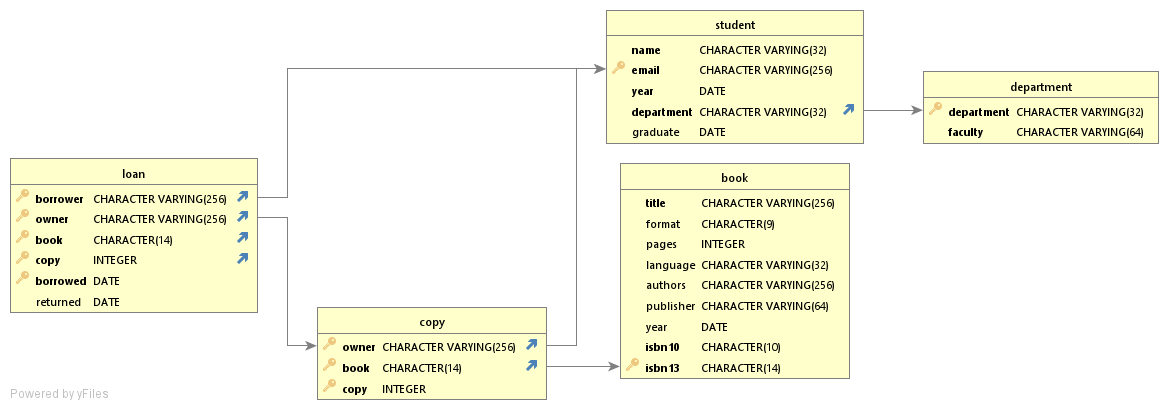
\includegraphics[width=1\textwidth]{t1/images/t1-end.png}
	\end{figure}
	(plotted by DbVisualizer)
\end{frame}

\section*{Question 1 Simple Queries}

\begin{frame}[fragile]{Question 1 (a-c)}
	(a) Print the different departments.\\ \vspace{5pt}
	(b) Print the different departments in which students are enrolled. \\ \vspace{5pt}
	(c) Let us check the integrity of the data. Print the emails of the students who borrowed or lent a copy of a book before they joined the university. There should not be any. Use a simple query.  
\end{frame}

\begin{frame}[fragile]{Solution 1 (a, b)}
(a) Print the different departments.\\ \vspace{5pt}

\begin{lstlisting}		
SELECT d.department FROM department d;
\end{lstlisting}

\textcolor{red}{13} row are returned.
Notice that the query does not require \texttt{DISTINCT} to eliminate duplicates. Duplicates are guaranteed not to occur because \texttt{department} is the \texttt{PRIMARY KEY} of the table \texttt{department}. \vspace{10pt}

(b) Print the different departments in which students are enrolled. \\ \vspace{5pt}

\begin{lstlisting}
SELECT DISTINCT s.department FROM student s;
\end{lstlisting}

\textcolor{red}{13} row are returned.
There could be departments in which no student is enrolled. This is the case of the department of \texttt{Undecidable Computations}.  We need to look into the \texttt{student} table.
\\\vspace{10pt}
\textcolor{brown}{\textbf{Do these two questions return the exactly SAME outputs?}}

\end{frame}

\begin{frame}[fragile]{Solution 1 (a, b) Cont.}

\begin{block}{Notice}
	The outputs of these two queries have the same contents but with different orders.
\end{block}\vspace{10pt}

	\begin{columns}
		\column{0.45\textwidth}
		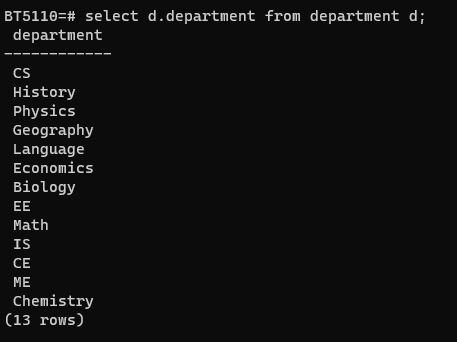
\includegraphics[width=\textwidth]{t2/images/t2-1a.png}
		
		\column{0.5\textwidth}
		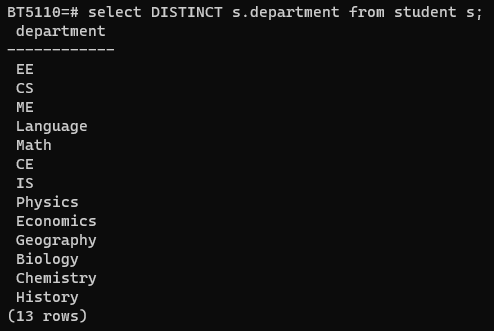
\includegraphics[width=\textwidth]{t2/images/t2-1b.png}
	\end{columns}

\vspace{5pt}
\textbf{Extra}: We can add ``\texttt{ORDER BY d.department ASC}'' in 1(a) and ``\texttt{ORDER BY s.department ASC}'' in 1(b) to make these two outputs same in ordering.
	
\end{frame}

\begin{frame}[fragile]{Solution 1 (c)}
(c) Let us check the integrity of the data. Print the emails of the students who borrowed or lent a copy of a book before they joined the university. \textbf{There should not be any.} Use a simple query.\\\vspace{10pt}

\textbf{Solution:} Don't forget to consider both \textit{borrowing} and \textit{lending} scenarios.\\

\begin{lstlisting}
SELECT DISTINCT s.email FROM loan l, student s 
WHERE (s.email = l.borrower AND l.borrowed < s.year) 
	OR (s.email = l.owner AND l.borrowed < s.year);
\end{lstlisting}
\end{frame}


\begin{frame}[fragile]{Question 1 (d)}

For each copy that has been borrowed and returned, print the \textbf{duration} of the loan. Order the results in \textbf{ascending} order of the ISBN13 and \textbf{descending} order of duration.  \\ \vspace{15pt}

\textcolor{brown}{\textbf{How can the duration be derived? Can we use ``returned - borrowed AS duration''?}}\\ \vspace{5pt}

\begin{lstlisting}
	SELECT book, returned - borrowed AS duration 
	FROM loan
	ORDER BY book ASC, duration DESC;
\end{lstlisting}

\textcolor{brown}{\textbf{Any issue in the code above?}}
\end{frame}

\begin{frame}[fragile]{Solution 1 (d)}
	Let's manually exclude NULL values in \texttt{returned} column:\\
	\begin{lstlisting}
		SELECT book, returned - borrowed + 1 AS duration 
		FROM loan
		WHERE NOT (returned ISNULL)
		ORDER BY book ASC, duration DESC;
	\end{lstlisting}

\begin{block}{Notice}
\texttt{ASC} is the default, but it is strongly recommended to indicate it for clarity.
\end{block}	

\textbf{Result}: \textcolor{red}{4871} rows are returned ($\neq$ number of rows in table \texttt{loan}).

\end{frame}

\begin{frame}[fragile]{Solution 1 (d) Cont.}

\textcolor{brown}{\textbf{What if the question ask like follows:}} \\ \vspace{5pt}

For each copy \textcolor{red}{\st{that has been borrowed and returned}}~\textcolor{ForestGreen}{record in the \texttt{loan} table}, print the \textbf{duration} of the loan. Order the results in \textbf{ascending} order of the ISBN13 and \textbf{descending} order of duration.  \\ \vspace{15pt}
% We do have loan records with NULL returned value! We need to count them in.
	
\end{frame}

\begin{frame}[fragile]{Solution 1 (d) Cont.}
	
Notice that the duration can be \textbf{null} if the book has not been returned yet. To answer this question, you need to calculate the duration until a specific date (e.g., December 31, 2010) to include the books that have not been returned yet. \vspace{10pt}
	
\begin{lstlisting}
SELECT book, ((CASE	WHEN returned ISNULL 
		THEN '2010-12-31'
		ELSE returned END) - borrowed + 1) AS duration 
	FROM loan
	ORDER BY book ASC, duration ASC;
\end{lstlisting}
\vspace{10pt}
 
\textbf{Result}: \textcolor{red}{4976} rows are returned (= number of rows in table \texttt{loan})

\begin{exampleblock}{}
	You can also use a Postgres reserved command ``\texttt{current\_date}'' to obtain the date of today (by doing this, some \texttt{duration} values will be huge). 
\end{exampleblock}	
\end{frame}


\begin{frame}[fragile]{Question 1 (e)}

For each loan of a book published by Wiley that has not been returned, print the title of the book, the name and faculty of the owner and the name and faculty of the borrower. Use \textbf{CROSS JOIN}.
\vspace{15pt}
%\begin{figure}
%	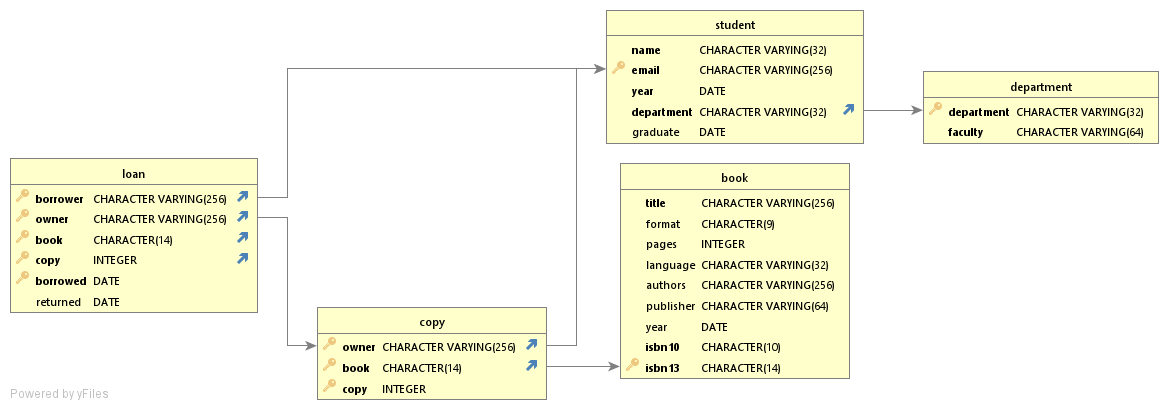
\includegraphics[width=1\textwidth]{t1/images/t1-end.png}
%\end{figure}

\textcolor{red}{Let's do 4 steps to form your query as follows:\\\vspace{5pt}
Step (1) FIND all output columns;\\
Step (2) IDENTIFY all value constraints;\\
Step (3) CONFIRM all tables involved;\\
Step (4) CONNECT tables involved (w. necessary relation constraints).}
\vspace{15pt}
\begin{center}
*** LIVE DEMO ***
\end{center}
\end{frame}

\begin{comment}
\begin{frame}[fragile]{Solution 1 (e)}

We join primary keys and foreign keys to \textit{\textbf{stitch}} tables together properly. 

\begin{lstlisting}
SELECT b.title, 
	s1.name AS ownername, 
	d1.faculty AS ownerFaculty, 
	s2.name AS borrowername, 
	d2.faculty AS  borrowerfaculty
FROM loan l, book b,  copy c, 
	student s1, student s2, 
	department d1, department d2
WHERE c.book = b.ISBN13
	AND c.book = l.book 
	AND c.copy = l.copy 
	AND c.owner = l.owner
	AND l.owner = s1.email
	AND l.borrower = s2.email
	AND s1.department = d1.department
	AND s2.department = d2.department
	AND b.publisher ='Wiley'
	AND l.returned ISNULL;
\end{lstlisting}

\textcolor{red}{\textbf{10}} rows are returned.

\end{frame}
\end{comment}

\begin{frame}[fragile]{Solution 1 (e)}

We join primary keys and foreign keys to \textit{\textbf{stitch}} tables together properly. 
	
\begin{figure}
	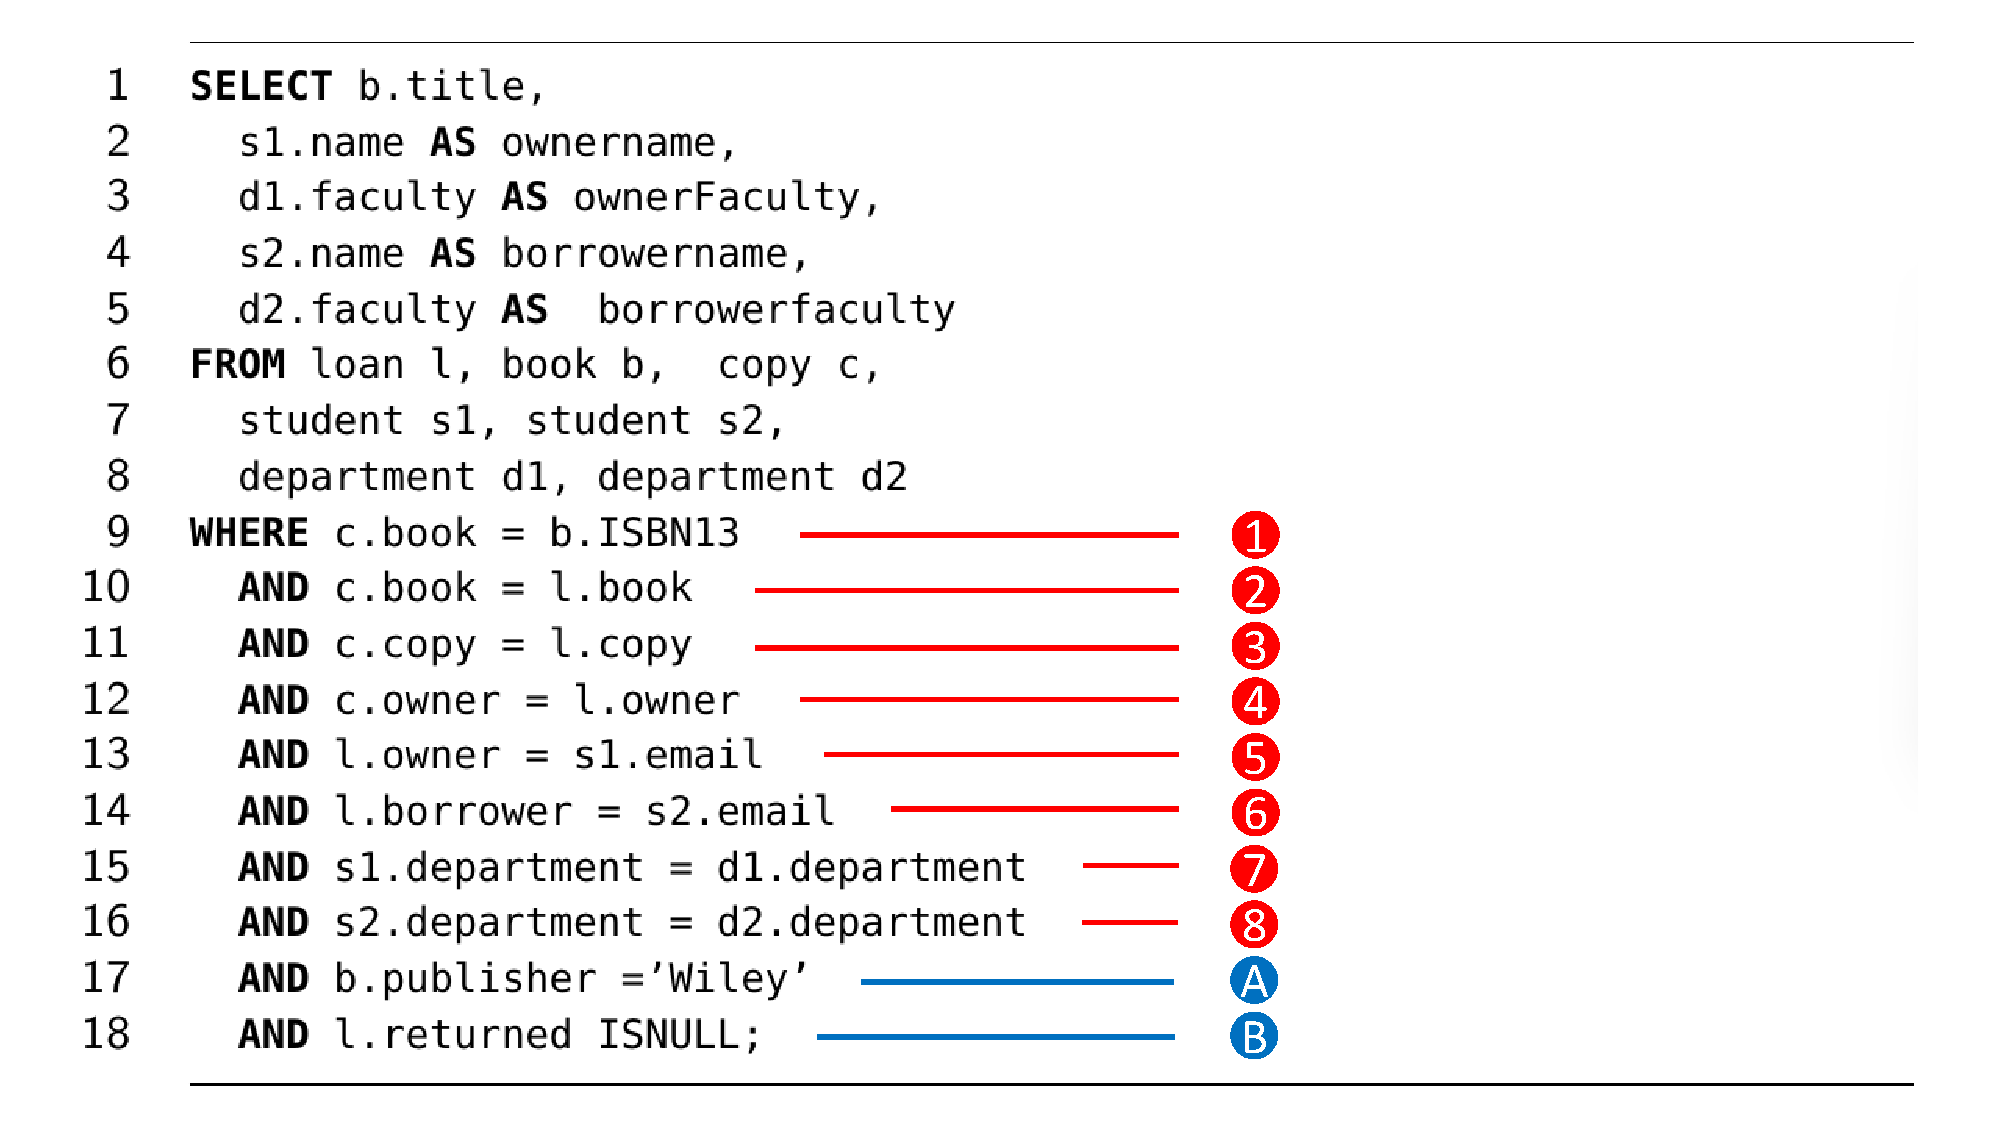
\includegraphics[width=1\textwidth]{t2/images/t2-q1e.pdf}
\end{figure}

\textcolor{red}{\textbf{10}} rows are returned.

\end{frame}

\begin{frame}[fragile]{Solution 1 (e) Cont.}
You can omit the table \texttt{copy}  and the \texttt{copy} column since the existence of the corresponding rows and values is guaranteed by design and by the foreign and primary key constraints.
	
\begin{lstlisting}
SELECT b.title, 
	s1.name AS ownername, 
	d1.faculty AS ownerFaculty, 
	s2.name AS borrowername, 
	d2.faculty AS  borrowerfaculty
FROM loan l, book b,  
	student s1, student s2, 
	department d1, department d2
WHERE l.book = b.ISBN13
	AND l.owner = s1.email
	AND l.borrower = s2.email
	AND s1.department = d1.department
	AND s2.department = d2.department
	AND b.publisher ='Wiley'
	AND l.returned ISNULL;
\end{lstlisting}

\end{frame}

\section*{Question 2 Algebraic Queries}

\begin{frame}[fragile]{Question 2 (a)}
For each loan of a book published by Wiley that has not been returned, print the title of the book, the name and faculty of the owner and the name and faculty of the borrower. Use \textbf{INNER JOIN}.

\begin{figure}
	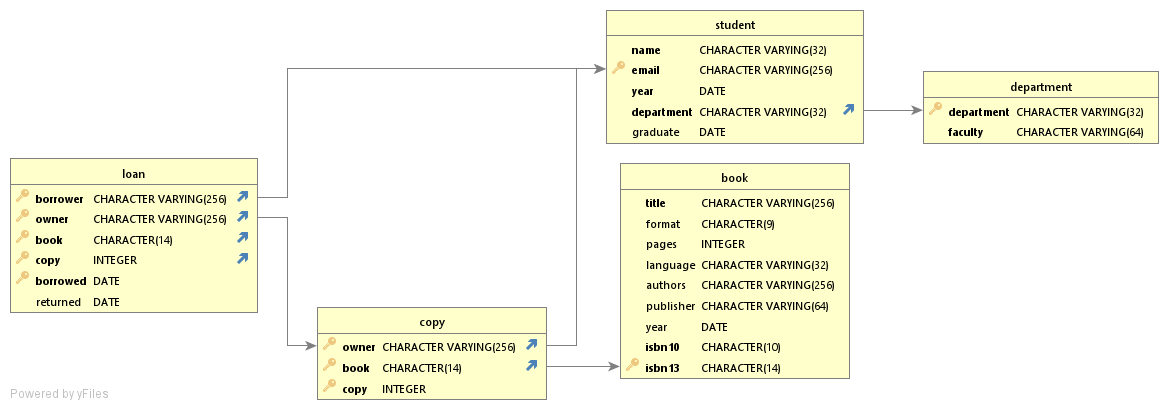
\includegraphics[width=1\textwidth]{t1/images/t1-end.png}
\end{figure}

\textcolor{brown}{This is the same question with Q1(e), but requires you to use INNER JOIN.}
\end{frame}

\begin{frame}[fragile]{Solution 2 (a)}
Let's convert the solution of Q1(e) now!\\
\vspace{10pt}

\begin{columns}
\column{0.52\textwidth}

\begin{lstlisting}
SELECT b.title, 
	s1.name AS ownername, 
	d1.faculty AS ownerFaculty, 
	s2.name AS borrowername, 
	d2.faculty AS  borrowerfaculty
FROM loan l, book b,  
	student s1, student s2, 
	department d1, department d2
WHERE l.book = b.ISBN13
	AND l.owner = s1.email
	AND l.borrower = s2.email
	AND s1.department = d1.department
	AND s2.department = d2.department
	AND b.publisher ='Wiley'
	AND l.returned ISNULL;
\end{lstlisting}

\column{0.45\textwidth}
\begin{lstlisting}
SELECT b.title, 
	s1.name AS ownername, 
	d1.faculty AS ownerFaculty, 
	s2.name AS borrowername, 
	d2.faculty AS  borrowerfaculty
FROM loan l 
	INNER JOIN ____ ON ________
	INNER JOIN ____ ON ________
	INNER JOIN ____ ON ________
	INNER JOIN ____ ON ________
	INNER JOIN ____ ON ________
WHERE b.publisher ='Wiley'
	AND l.returned ISNULL;
\end{lstlisting}
\end{columns}
	
\end{frame}

\begin{frame}[fragile]{Solution 2 (a) Cont.}

You can omit the table \texttt{copy} and the \texttt{copy} column since the existence of the corresponding rows and values is guaranteed by design and by the foreign and primary key constraints.

\begin{lstlisting}
SELECT b.title, 
	s1.name AS ownername, 
	d1.faculty AS ownerFaculty, 
	s2.name AS borrowername, 
	d2.faculty AS  borrowerfaculty
FROM loan l 
	INNER JOIN book b ON l.book=b.ISBN13
	INNER JOIN student s1 ON l.owner = s1.email
	INNER JOIN student s2 ON l.borrower = s2.email
	INNER JOIN department d1 ON s1.department = d1.department
	INNER JOIN department d2 ON s2.department = d2.department
WHERE  b.publisher ='Wiley'
	AND l.returned ISNULL;
\end{lstlisting} 

\textcolor{red}{\textbf{10}} rows are returned.
\end{frame}

\begin{frame}[fragile]{Solution 2 (a) Cont.}
	
	The code below is \textbf{without omitting table \texttt{copy}}. The simplified version is shown on the previous slide.	
	
	\begin{lstlisting}
		SELECT b.title ,
		s1. name AS ownername ,
		d1. faculty AS ownerFaculty ,
		s2. name AS borrowername ,
		d2. faculty AS borrowerfaculty
		FROM loan l
		INNER JOIN book b ON l. book = b. ISBN13
		INNER JOIN copy c ON c. book = l. book
		AND c. copy = l. copy AND c. owner = l. owner
		INNER JOIN student s1 ON l. owner = s1. email
		INNER JOIN student s2 ON l. borrower = s2. email
		INNER JOIN department d1 ON s1. department = d1. department
		INNER JOIN department d2 ON s2. department = d2. department
		WHERE b. publisher ='Wiley'
		AND l. returned ISNULL ;
	\end{lstlisting} 
	
\end{frame}
	
\begin{frame}[fragile]{Question 2 (b)}
Print the emails of the different students who borrowed or lent a copy of a book on the day that they joined the university. Use an algebra\"{\i}c query.\\
\vspace{10pt}
\textcolor{brown}{\textbf{Set operations (UNION, INTERSECT and EXCEPT) could help to address this question.}}
\end{frame}

\begin{frame}[fragile]{Solution 2 (b)}

\begin{lstlisting}
SELECT  s.email 
FROM loan l, student s 
WHERE s.email = l.borrower AND l.borrowed = s.year
UNION
SELECT  s.email 
FROM loan l, student s 
WHERE s.email = l.owner AND l.borrowed = s.year;
\end{lstlisting}

\textcolor{red}{\textbf{19}} rows are returned.\\
\vspace{5pt}
\texttt{DISTINCT} is not needed because \texttt{UNION}  eliminates duplicates (so do \texttt{INTERSECT}, \texttt{EXCEPT} and \texttt{MINUS}). 

\end{frame}

\begin{frame}[fragile]{Question 2 (b) Cont.}
There is an alternative (simple) way to write the query, without SET operations.\\
\vspace{10pt}
The corresponding simple query is generally preferable.

\begin{lstlisting}
SELECT DISTINCT s.email 
FROM loan l,  student s 
WHERE (s.email = l.borrower OR s.email = l.owner) 
	AND l.borrowed = s.year;
\end{lstlisting}

\begin{alertblock}{Notice}
The simple query requires an explicit \texttt{DISTINCT}.	
\end{alertblock}

\end{frame}

\begin{frame}[fragile]{Question 2 (c)}
Print the emails of the different students who borrowed and lent a copy of a book on the day that they joined the university. Use an algebra\"{\i}c query.\\
\vspace{10pt}
\textcolor{brown}{\textbf{Which set operation (UNION, INTERSECT and EXCEPT) should we use for this question?}}
\end{frame}

\begin{frame}[fragile]{Solution 2 (c)}
\begin{lstlisting}
SELECT  s.email 
FROM loan l, student s 
WHERE s.email = l.borrower AND l.borrowed = s.year
INTERSECT
SELECT  s.email 
FROM loan l, student s 
WHERE s.email = l.owner AND l.borrowed = s.year;
\end{lstlisting}
\vspace{5pt}
\textcolor{red}{\textbf{4}} rows are returned.\\
\vspace{10pt}
Note that the corresponding simple query is more \textit{\textbf{complicated}}. It needs \textbf{\textit{two}} \texttt{loan} tables.

\begin{lstlisting}
SELECT DISTINCT s.email 
FROM loan l1, loan l2, student s 
WHERE s.email = l1.borrower AND l1.borrowed = s.year 
AND s.email = l2.owner AND l2.borrowed = s.year;
\end{lstlisting}
\end{frame}

\begin{frame}[fragile]{Question 2 (d)}
Print the emails of the students who borrowed but did not lend a copy of a book on the day that they joined the university. Use an algebra\"{\i}c query.\\
\vspace{10pt}
\textcolor{brown}{\textbf{Which set operation should we use for this question?}}
\end{frame}

\begin{frame}[fragile]{Solution 2 (d)}
\begin{lstlisting}
SELECT  s.email 
FROM loan l, student s 
WHERE s.email = l.borrower AND l.borrowed = s.year
EXCEPT
SELECT  s.email 
FROM loan l, student s 
WHERE s.email = l.owner AND l.borrowed = s.year;
\end{lstlisting}

\vspace{5pt}
\textcolor{red}{\textbf{9}} rows are returned.\\
\vspace{10pt}
There is no corresponding simple query. We would need to use nested or aggregate queries for this type of questions.
\end{frame}

\begin{frame}[fragile]{Question 2 (e)}
Print the ISBN13 of the books that have never been borrowed. Use an algebra\"{\i}c query.
\end{frame}

\begin{frame}[fragile]{Solution 2 (e)}
\textbf{Solution}:
\begin{lstlisting}
SELECT b.ISBN13 
FROM book b
EXCEPT
SELECT l.book 
FROM loan l;
\end{lstlisting}

\vspace{5pt}
\textcolor{red}{\textbf{0}} rows are returned.\\
\vspace{10pt}
or, using an \textit{OUTER JOIN}, which introduces NULL values,

\begin{lstlisting}
SELECT b.ISBN13 
FROM book b LEFT OUTER JOIN loan l ON b.isbn13 = l.book
WHERE l.book ISNULL;
\end{lstlisting}

There is no corresponding simple query. We would need to use nested or aggregate queries for this type of questions.

\end{frame}

\begin{frame}{}
\centering  
For any further question, please feel free to email me:\vspace{10pt}

huasong.meng@u.nus.edu \vspace{20pt}

\begin{tcolorbox}
	\begin{center}
		\textcolor{red}{Copyright 2021 Mark H. Meng. All rights reserved.}
	\end{center}
\end{tcolorbox}

\end{frame}